
% ------------------------------------------------------------------------------------------------------------------------------------------------
\chapter{System design}
\label{chap:system-design}

The system is designed with both: asynchronous and distributed approaches in mind. In order to achieve high asynchronicity between obtaining new reference data, and running jobs such as ``\textit{compare video1 with the reference database}'', the system was split into two primary components:

\begin{itemize}
  \item \textbf{Loader} -- responsible for obtaining more and more reference material. It persists and initially processes the videos, as well as any related metadata. In a the real world, such reference data is usually provided by partners, such as movie or television companies,
  \item \textbf{Analyser} -- responsible for preparing and scheduling job pipelines for execution on top of the Hadoop cluster and reference databases.
\end{itemize}

To further illustrate the separate components and their interactions Figure \ref{fig:system-overview} shows the different interactions within the system.

\begin{figure}[hc!]
 \centering
  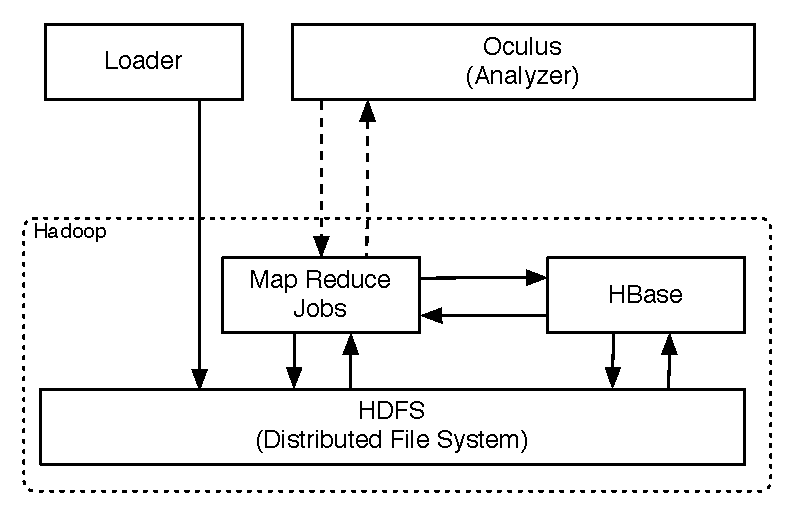
\includegraphics[scale=0.9]{./diagrams/high-level-system.pdf}
  \caption{High level overview of the system's architecture}
  \label{fig:system-overview}
\end{figure}

This section will focus on describing the general design of both systems, first the Loader's actor-based cluster model, and then the Analyser's Hadoop-backed batch processing cluster.

% ------------------------------------------------------------------------------------------------------------------------------------------------
\newpage
\section{Loader}
\label{sec:loader-basics}
The Loader component is responsible for obtaining as much as possible ``reference data'', by which video material from sites such as \textit{youtube.com} or video hosting sites is meant. Please note that for the sake of this thesis (and legal safety) the downloaded content was limited to movie trailers (which are freely available on-line) as well as series opening or ending sequences.

While the Loader system will be referred to from here on in singular, it should be noted that in fact there are multiple instances of it running in the cluster. Thanks to the use of Akka's \textit{Cluster} module \cite{akka-cluster}, it was also fairly easy to distribute actors among multiple physical nodes in the cluster, allowing the actor system to utilise the entire cluster's processing power. The use of messaging as default and only mean of communication with actors allowed to easily transition into the clustered model, where communication would he handled over the network, from a previously local-only model.

\subsection{Types of Actors used in the system}
\label{sec:types-of-actors}

The system consists of 4 types of Actors. Each of them has multiple instances which are spread out on many nodes in the cluster. Some tasks can only be sent to local Actors (any work requiring an already downloaded file), but messages related to crawling and initially downloading the video material can be spread throughout the cluster. 

The following Actor descriptions are aimed at explaining the protocols used for communication between them in the running system. These are very important as actors can communicate only via sending and receiving messages, and can not provide any type signatures that would help to identify what messages they can respond to. The also do not have methods that can be called directly on them -- this is a direct result of implementing actor model based concurrency, which would not be able to hold in face of direct access to an actors state.

will now briefly describe the different Actor roles that exist in the system and then explain the interactions between then on an example.

\begin{itemize}
  \item \textbf{YouTubeCrawlActor} -- is capable of fetching and YouTube websites and and crawling of ``related video
                                      sites'' (\verb|Crawl(siteId: String)|). It also sends messages that trigger the 
                                      download process by sending \verb|Download(movieId: String)| messages,
    \subitem  \textbf{receives:}
      \subsubitem \verb|Crawl(siteId: String)| messages,
    \subitem  \textbf{sends:}
      \subsubitem 0 or n -- \verb|Crawl(siteId: String)| - where n is the number of ``related video'' links found on the site.
                                                           If crawling is turned off, no messages will be sent,

  \item \textbf{DownloadActor} -- downloads the movie from youtube in it's original format (in the presence of many formats, 
                                the highest quality file will be downloaded). metadata,
    \subitem  \textbf{receives:}
      \subsubitem \verb|Download(siteId: String)| messages,
                      
                      \newpage          
  \item \textbf{ConversionActor} -- converts the downloaded video material into raw frame data (bitmaps),
    \subitem  \textbf{receives:}
      \subsubitem \verb|Convert(localVideoFile: java.util.File)| -- which must come from a local Actor, since the path refers to the local file system,
    \subitem  \textbf{sends:}
      \subsubitem 1 -- \verb|Upload(framesDirectory: java.util.File)| -- when the finished converting to bitmaps, it will send and \verb|Upload| message to one of the\verb|HDFSUploadActors|, pointing to the directory where the output bitmaps have been written,
                                                                    
  \item \textbf{HDFSUploadActor} -- stores the sequence of bitmaps in Hadoop. This includes converting a series of 
                                  relatively small (around 2MB per frame) files into one Sequence File on HDFS. Sequence Files and the need for their use
                                  will be explained in detail in section \ref{sec:sequence-files},
  \subitem \textbf{receives:}
    \subsubitem \verb|Upload(framesDirectory: java.util.File)| -- pointing to a local directory where the bitmap files have been stored.
                                                                 This message must come from a local actor, since the path refers to the local file system,
    \subitem  \textbf{sends:}
      \subsubitem 0 or 1 -- \verb|ConfirmUpload(localFile: java.util.File)| -- sent back to the sender that requested the video to be uploaded.
\end{itemize}

Using these Actors and protocols between them, the application is able to progress safely without the possibility of getting stuck in a dead (or live) lock. 

While discussing there protocols one should also mention that the messages that can be received and sent by Actors are not possible to verify using static typing -- an Actor can receive a message of ``Any'' type, and in case of not being able to act upon it - it will drop the message, but the delivery still happens.
This is an inherent property of the Actor Model of concurrency -- which is why in such systems explaining the flows of messages and Actors present in the system is of such importance. Having this in mind, the next Section (\ref{sec:obtaining-reference-material}) will focus on explaining one such message flow within the system.

% -------------------------------------------------------------------------------------------------------------------------------------------------
\subsection{Obtaining reference video material}
\label{sec:obtaining-reference-material}
This section wills discuss the process of obtaining video material by the Loader subsystem, as well as explain which parts can be executed on different nodes (node-01, node-02, node-N) of the cluster. Figure \ref{fig:high-level-loader} together with the flow description in this section aim to provide the necessary high-level overview of the system's execution flow.

\begin{figure}[ch!]
  \centering
  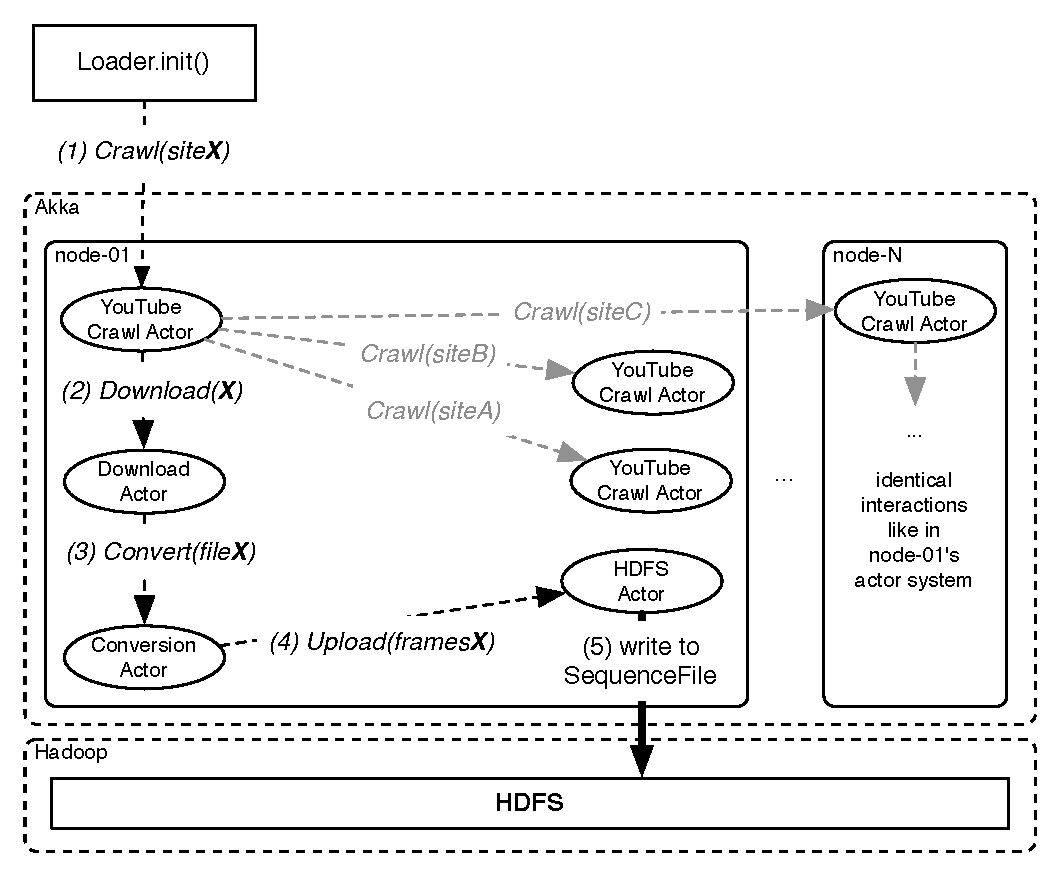
\includegraphics[scale=0.9]{img/loader-high-level.pdf}
  \caption{Overview of messages passed within the Loader's actor system. Greyed out messages are also sent, but are not on the critical path leading to obtaining material from \textit{siteX} into HDFS.}
  \label{fig:high-level-loader}
\end{figure}

\subsubsection{Step 1 - \textit{Crawl} messages}
The initiating message for each flow within the Loader is a \textit{Crawl(siteUrl)}, where siteUrl is a valid youtube video url.
The receiving YouTubeCrawlActor will react to such message by fetching and extracting the related video site urls and will forward those using the same kind of \textit{Crawl} messages. The second, yet most important, reaction is sending a \textit{Download(movieId)} message to an instance of an DownloadActor -- it  can reside on any node in the cluster, which allows us to spread the down-link utilisation between different nodes in the cluster.

It is worth pointing out that the receivers of these messages can be \textit{remote} Actors, that is, can be located on a different node in the Cluster than the sender. In order to guarantee spreading of the load among the many actors within the system (across nodes in the cluster), a routing strategy called ``Smallest Inbox Routing'' was used. This technique uses a special ''Router Actor'' which is responsible for a number of Routees (target Actors), and decides to deliver a message only to the Actor who has the smallest amount of messages ''not yet processed'' (which are kept in an Queue called the ''Inbox'', hence the strategy's name).

\subsubsection{Step 2 - \textit{Download} messages}
In the second step an \textit{YouTubeDownloadActor} instance receives a message asking it to download a movie.
It does so by invoking the native app \textit{youtube-dl}, which is an open source program specialised in downloading movies from YouTube.
Other than the video file (in an open source format) we also download a metadata description during this step, such metadata includes for example the date of publication, author, title and description of the movie. From this message including, all messages will be routed only to Actors local to the current node, because messages include \textit{File} objects, pointing to locations on-disk.

The metadata is then used to determine if it can be used in the context of this work, as only movie trailers and and opening / ending sequences are downloaded into the Oculus system. If the content is OK to use, the Actor sends an \textit{Convert(movieLocation)} message to an instance of \textit{ConversionActor}.

\subsubsection{Step 3 - \textit{Convert} messages}
The next step is executed by an instance of an \textit{ConversionActor} receiving an \textit{Convert(file)} message from another (local) Actor. The conversion phase will extract raw frame data from the incoming movie, and write those as plain bitmaps (not compressed) to files (one per each frame) into a specified target directory. The reason for not using a compressed lossless image format here is that all algorithms that the system will be dealing with later on are dealing with the raw image data, so we can avoid having to go over un-compression phases each time we will process a frame. Having that said, the storage format used for storing these files on HDFS provides build in compression (if enabled), and it should be preferred in this case as it is transparent for the application, easing development of Map Reduce jobs in the Analyser system immensely.

The conversion from movie to raw bitmaps is performed by running an native application called \verb|ffmpeg| \cite{ffmpeg} instance (an de facto standard tool for such media operations), by forking a process from within the Actor. The CPU usage of running this extraction process easily reaches 100\% of the available resources, restricting the number of Conversion Actors per node is limited to only 1 per node, allowing ffmpeg to consume all available resources and finish extracting the data sooner. The actor will block until the process completes, and will then continue by sending an \textit{Upload(bitmapDirectory)} message to one of the \textit{HDFSUploadActors}.

\subsubsection{Step 4 \& 5 - \textit{Upload} messages}
The last step is an \textit{HDFSUploadActor} receiving an \textit{Upload(bitmapDirectory)} message which triggers it to connect to HDFS and start writing the bitmap data contained in the given directory to HDFS. The format of the generated data is as previously mentioned one file per frame of video, which averages to around 2MB per frame (depending on the movie resolution).

In this step the important part is that it does not write these files 1:1 onto HDFS, but instead writes into one file, using a hadoop specific storage format called ``Sequence File'', which allows for more efficient storage and latter retrieval of this data. Sequence Files, the need and benefits gained by using them as storage format for ''frame by frame'' data will be discussed in Section \ref{sec:sequence-files}.

This write terminates the operations performed on one movie by the Loader. All other operations will be performed by the Analyser by running Map Reduce jobs on Sequence Files prepared in the above flow.

\subsection{Loader design summary}
As was explained in the previous sections the Loader is designed as a fully asynchronous system, composed of Actors performing very specific tasks. All communication between the Actors is implemented as message passing, which allows for \textit{location transparency} between the Actors -- this property has been utilised to spread the work-load between multiple nodes in a clustered environment, enabling the work to be completed faster than only utilising a single node.

A detailed discussion of the Cluster's scalability and patterns applied in order to provide ad-hoc joining of nodes to the computation cluster can be found in Section \ref{chap:perf-scalability}: ``Scaling out the Actor system based Cluster''.

% ------------------------------------------------------------------------------------------------------------------------------------------------
\section{Analyser}
\label{sec:analyser}
The analyser component is responsible for orchestrating Map Reduce jobs and submitting them to the cluster. Results of jobs are written to either HBase or plain TSV (\textit{Tab Separated Values}) files. Figure \ref{fig:analyser-high-level} depicts the typical execution flow of an analysis process issued by Oculus.

\begin{figure}[ch!]
  \centering
  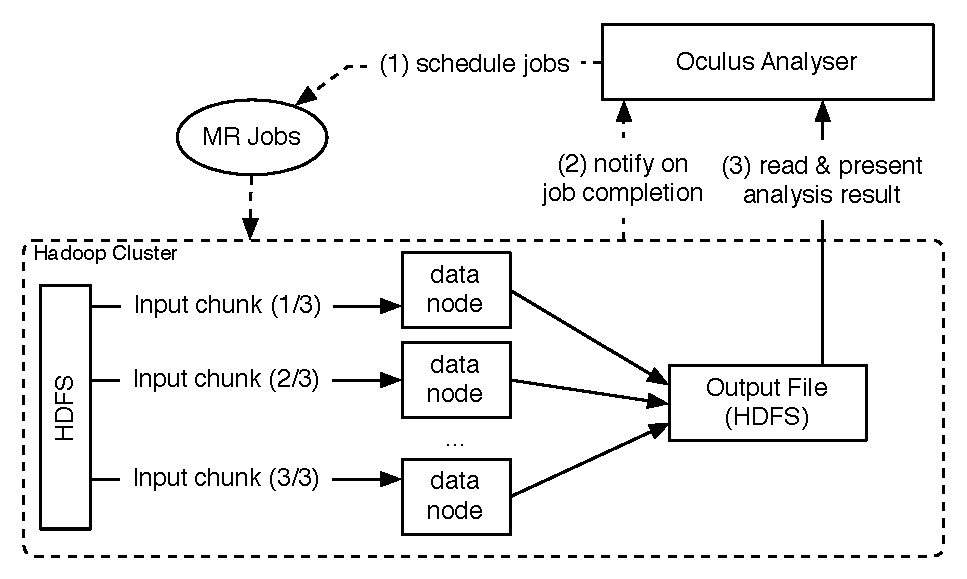
\includegraphics[scale=0.9]{img/analyser-high-level}
  \caption{Overview of the Analyser's execution flow, when working with}
  \label{fig:analyser-high-level}
\end{figure}

In step 1 the \textit{job pipeline} is being prepared by the program by aggregating required metadata and preparing the job pipeline, which often consists of more than just one Map Reduce job -- in fact, most analysis jobs performed by Oculus require at least 3 or more Map Reduce jobs to be issued to the cluster. It is important to note that some of these jobs may be dependent on another task's output and this cannot be run in parallel. On the other hand -- if a job requires calculating all histograms for all frames of a movie as well as calculating something different for each of these frames -- these jobs can be executed in parallel and will benefit from the large number of data nodes which can execute these jobs.

The 2nd step on Figure \ref{fig:analyser-high-level} is important because Oculus may react by launching another analysis job based on the notification that one pipeline has completed. This allows the system to keep the different pipelines separate, and trigger them reactively when for example all it's dependencies have been computed in another pipeline.

For most applications though the 3rd step in a typical Oculus Job would be to read and present top N results to the issuer of the job, which for a question like ``Which movie is similar to this one?'' would be the top N most similar movies (their names, identifiers as well as match percentage).

The following sections (\ref{sec:deployment-strategy}, \ref{sec:scalding-jobs}) will introduce the cluster deployment as well as how Jobs are implemented on top of it, in order to parallelise the job's execution as much as possible.



% ------------------------------------------------------------------------------------------------------------------------------------------------
\subsection{Hadoop Cluster deployment strategy}
\label{sec:deployment-strategy}

Since the Analyser is most dependent on the Hadoop cluster's deployment this section aims to introduce the cluster's components and initial (3 node) setup. 

While this section only only introduces the various components of the cluster and it's initial deployment, chapter \ref{chap:perf-scalability} (``Cluster scaling and performance analysis'') revisits this topic and will focus on details such as cluster configuration options as well as influence of the number of participating nodes in the cluster on total computation times will be measured and tuned to increase the cluster's efficiency.

\subsubsection{Initial Hadoop cluster deployment}

The Hadoop deployment described in this subsection will focus on two elements of the Hadoop ecosystem - the Hadoop Distributed File system (HDFS) and the Hadoop Map Reduce Runtime.

The minimal hadoop deployment consists of \textit{5 individual processes}, each with an assigned and very specific role in the clusters functioning. These processes can be classified as running along side the NameNode or DataNodes. This distinction should be clear after listing the names and features of these processes.

There are 3 processes associated with the ``master node'', namely: the NameNode, the SecondaryNameNode and the JobTracker which is responsible for coordination of HDFS operations and Map Reduce Job scheduling:

\begin{itemize}
  \item \textbf{NameNode} (HDFS) -- responsible for mapping logical file paths to their locations on DataNodes within 
                                    the cluster. This component was a Single Point of Failure (SPOF) on Hadoop clusters 
                                    until version 2.0 implemented the so called High Availability (HA) module, which 
                                    allows the cluster to run a second (not to be confused with \textit{secondary}) 
                                    NameNode in the cluster in the case the primary would fail. The HA module was not 
                                    used during this thesis, as it was not required to ensure the cluster's high 
                                    availability as the data could always be easily obtained again,
  \item \textbf{SecondaryNameNode} (HDFS) -- responsible for a process called ``checkpointing'' of the NameNode's
                                            fsimage and it's edit-log. It's name may be very misleading, as at no point
                                            in time is the SecondaryNameNode able to take the primary NameNode's place -- 
                                            this can be only achieved by using the High Availability modules. Use of the 
                                            SecondaryNameNode though allows the NameNode to fail and re-join a running 
                                            cluster -- without the SecondaryNameNode that failed NameNode would have lost 
                                            all of it's file system state and a full HDFS restart (including all 
                                            datanodes) would be required,
  \item \textbf{JobTracker} (MapReduce) -- responsible for scheduling Map Reduce Jobs running in the cluster. It
                                           behaves like a queue, taking in Job requests and processes them in order (or    
                                           based on customisable strategies). It is also in contact with all TaskTrackers 
                                           (described below), which actually perform the work related to a MR Job, while 
                                           the JobTracker only gets and aggregates the job's progress. In case of failed 
                                           Jobs or Tasks it can also restart or redistribute the job to other DataNodes.
\end{itemize}

Secondly, the cluster contains 2 types of processes associated with \textit{slave} nodes. They are mostly responsible for ``the actual work'', whereas the processes running on the \textit{master} node can be seen as ''coordinators''. Each salve node in the cluster is running these processes:

\begin{itemize}
  \item \textbf{DataNode} (HDFS) -- responsible for the actual storage of data on HDFS. Data nodes themselves are not able 
                                    to correlate a path to a given file data block -- only the NameNode is able to 
                                    perform this lookup, which also means that in the case of the NameNode failing,
                                    the data stored on the DataNodes is temporarily unavailable. The DataNodes can talk 
                                    to each other in order to migrate and replicate the data blocks directly with each
                                    other, though this action has to be initialised by the NameNode,
  
  \item \textbf{TaskTracker} (MapReduce) -- responsible for scheduling and executing Jobs on a given DataNode. Tasks are
                                            chunks of work, issued by the JobTracker to TaskTrackers, which then handle
                                            their execution. Once all tasks for a given job are completed, the JobTracker 
                                            reacts by completing the overall job. A TaskTracker should be run on the same
                                            physical node as the DataNode, because then it can leverage this fact for
                                            node-local task execution.
\end{itemize}


\begin{figure}[ch!]
  \centering
  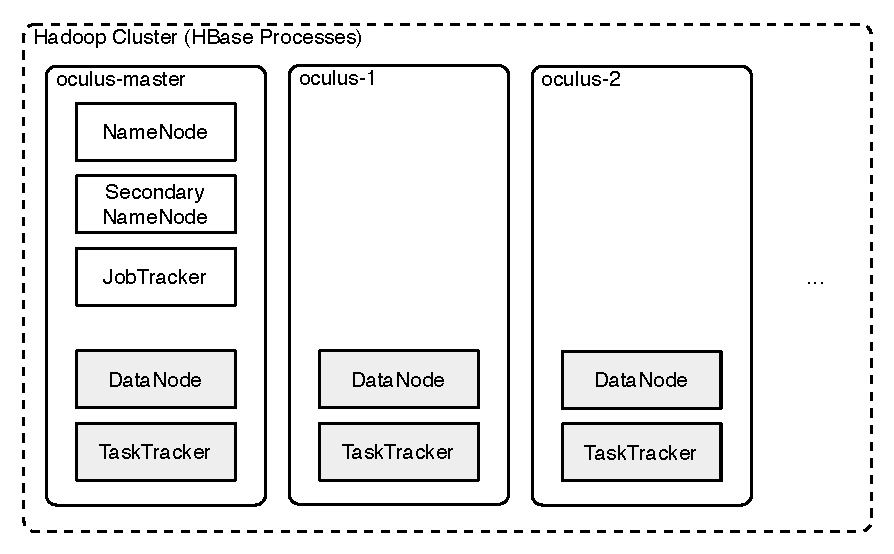
\includegraphics[width=0.90\textwidth]{img/hdfs-processes}
  \caption{Deployment diagram of the various HDFS processes within the initial 3-node cluster.}
  \label{fig:small-cluster-deployment}
\end{figure}

These 5 types of processes must be running in the cluster for Map Reduce jobs to be executable by the cluster. All nodes must be able to communicate with each other. Firstly, because the master node must be able to submit tasks to it's slave nodes (DataNodes) and secondly, because DataNodes must be able to communicate between themselves in order to replicate data among the cluster. Starting the cluster however does not require the administrator to start these processes on each of the machines separately -- as the master node is able to issue start/stop commands via \verb|ssh| to it's slave nodes. This also means that the slave nodes do not need to know about all their ``neighbours'', because the master node will inform the newly joined nodes about the cluster's current state and IP addresses of the remaining DataNodes.


\subsubsection{HBase deployment}
\label{sec:hbase-deployment}
Discussing the Hadoop cluster's deployment actually automatically covers part of the deployment information needed for the HBase cluster. The reason for this being, that the HBase cluster's equivalent of ``data node'', known as RegionServers must reside on the same physical nodes as HDFS's DataNodes.

HBase also has a clear separation between processes that are \textit{master} processes and \textit{slave} processes.
The master and coordination processes are:

\begin{itemize}
\item \textbf{HMaster} (HBase) -- responsible for all coordination of reads and writes to HBase. Although it may seem 
                                  that it might quickly become a bottleneck, since all client applications connect 
                                  directly to it, this is not the case. While clients indeed do connect directly to the 
                                  HMaster all read/write operations are performed directly between the client and             
                                  specific RegionServers which host the data that a given client query is touching,
\item \textbf{HQuorumPeer} (ZooKeeper) -- is HBase's wrapper around Apache ZooKeeper \cite{zoo-keeper}, which is a
                                          centralised multi-node quorum-based metadata storage service. ZooKeeper is used 
                                          for cluster management within HBase, and the HQuorumPeer serves as ''managed by
                                          HBase ZooKeeper cluster''. Thanks to HB running the ZK cluster by itself, for 
                                          small clusters (less than hundreds of nodes), it eases the administrative 
                                          overhead of managing another cluster manually. ZK is used to register and 
                                          auto-discover RegionServers, once they notify ZooKeeper of their existence.
\end{itemize}

While, exactly as with the NameNode in the case of HDFS, the HMaster should be a cluster-wide singleton, and serves as entry point for client applications for issuing reads and writes, the HQuorumPeer has to be run on multiple nodes. 

In initial configuration of the HBase cluster the HQuorumPeer was run on three nodes in the cluster. The reason for using 3 nodes to run the HQuorumPeer (ZooKeeper) processes is that, since ZK operates on a quorum it requires at least \verb|ceil(N/2)| nodes to be available to make progress. In an 3 node scenario, this means that the cluster will continue to work properly while at least \verb|ceil(3/2) = 2| nodes are available. In other words, setting up 3 nodes to run ZK, allows 1 node to fail, without stoping the entire cluster.

Continuing the discussion about process types running in the HBase cluster, the slave nodes require one type of component to be running:

\begin{itemize}
\item \textbf{HRegionServer} (HBase) -- responsible for processing client requests to read / write to HTables.
                                        The name ``Region'' mentioned in it's name refers to the fact that the
                                        \textit{row-key} space of a Table is split among multiple servers, so that when
                                        performing a full-scan filtering operation, multiple servers can perform the
                                        scanning \textit{in parallel} -- each for it's own section of the
                                        \textit{row-key} space. It must be running along side with a DataNode on the
                                        same physical server.
                                        
\end{itemize}

While the slave type of process is much simpler for HBase than for HDFS, it does have one additional requirement: an HRegionServer must be running on the same physical node as a HDFS DataNode. The reason behind this is that RegionServers store their assigned region's data on HDFS and by running it on the same node as a DataNode, all writes can be made locally -- without transferring the data over the network. Of course, if HDFS is configured to replicate it's data to multiple nodes -- it will, but this does not concern the HRegionServer.


\begin{figure}[ch!]
  \centering
  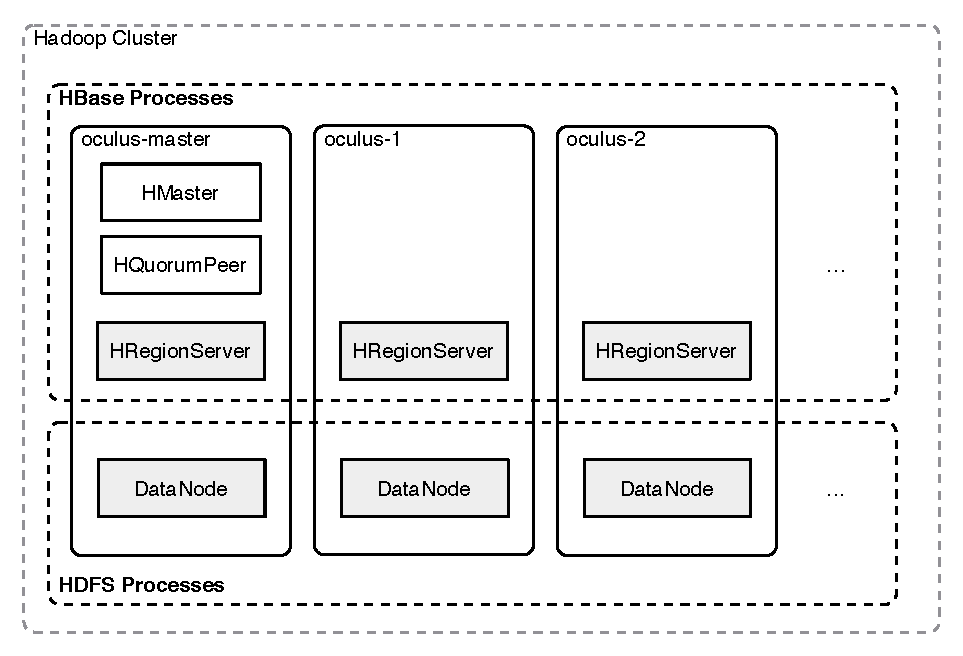
\includegraphics[width=0.95\textwidth]{img/hbase-processes}
  \caption{Deployment diagram of the various HBase processes within the initial 3-node cluster. DataNodes are not directly part of the HBase cluster, yet are required to be running on the same physical nodes as HRegionServers.}
  \label{fig:small-cluster-deployment}
\end{figure}

Having the HRegionServers deployed on the same nodes as DataNodes has another effect: all optimisations performed to HDFS and the DataNodes, will directly influence HBase's behaviour. One should also keep in mind that some features may seem to be duplicated among HDFS and HBase -- such as replication, which can be set up directly on HBase or HDFS. Configuring some of these settings in HBase rather than HDFS has the benefit of HBase being more aware of the structure of the data it is storing, whereas the same data carries nearly no meta information HDFS can use to redistribute it more efficiently. 
Namely, HBase can redistribute data related to Regions of HTables more efficiently, so that full scans on these tables can be parallelised more evenly and predictably.

All diagrams in this Section have included an ``$\cdots$'' marker, hinting at the possibility to add more nodes to the cluster. When scaling Hadoop clusters the only type of node that has to be added is the ''slave'' kind of node, which have been positioned right-most on each diagram. In fact, chapter Chapter \ref{chap:perf-scalability} will focus directly on scaling out these clusters, with one of the tests scaling it out to 10 nodes.

% ------------------------------------------------------------------------------------------------------------------------------------------------
\subsection{Defining Map Reduce Pipelines using Scalding and Cascading}
\label{sec:scalding-jobs}
The language and for implementing these processing pipelines used in this thesis was Scalding \cite{scalding}, which was already briefly introduced in Section \ref{sec:scalding-info}. The choice of Scalding, and not Hadoop's plain Map Reduce API, as a way of interacting with Hadoop jobs from Scala, strongly influenced by the increased understandability and ease of modifying complicated job pipelines. 

\subsubsection{Comparison of example Job implemented using Plain Hadoop and Scalding}

This section aims to demonstrate what gains using Scalding on top of Hadoop yields, by showing the smallest possible example of an Map Reduce Job, implemented using both plain Hadoop APIs and Scalding. One should remember that Scalding is not a different framework to  Hadoop, and in the end it will produce the exact same computations and classes (one instance of a \verb|Mapper| and one instance of a \verb|Reducer|).

The example shown on the below listings is a Hadoop equivalent of what programming languages aim to demonstrate using ``Hello World!'' applications -- it is a minimal piece of code showing the working of the given technology. The task to solve is defined as: ''\textit{Given a huge input text file, count the occurrences of each discrete word, and return a summary of these}''. As the aim of Hadoop is to leverage parallel computing, the classic method of implementing this task is to emit tuples of \verb|(word, 1)| for each word, then relying on Hadoops internal mechanisms to group tuples together by the first value (the \verb|word|), and reducing these into a tuple of \verb|(word, sum(1,1,1,...))|.

The difference in complexity should be obvious by comparing the Listings \ref{lst:hadoop-mr-map} and \ref{lst:hadoop-mr-reduce} represent the Map and Reduce classes which are used to represent the respectful Map and Reduce functions in the Java API, with Listing \ref{lst:simplest-scalding-job} which is the complete code for a job performing the exact same in Scalding's Scala Domain Specific Language. 

\begin{lstlisting}[caption={Word Count example Job -- Map implementation using plain Java Map Reduce API}, label={lst:hadoop-mr-map}]
public class Map 
    extends MapReduceBase 
    implements Mapper<LongWritable, Text, Text, IntWritable> {

 private final static IntWritable one = new IntWritable(1);
  private Text word = new Text();

  public void map(LongWritable key, 
                  Text value, OutputCollector<Text, IntWritable> output, 
                  Reporter reporter) throws IOException {
   String line = value.toString();
   StringTokenizer tokenizer = new StringTokenizer(line);
   while (tokenizer.hasMoreTokens()) {
    word.set(tokenizer.nextToken());
    output.collect(word, one);
   }
  }
}
\end{lstlisting}

\newpage
\begin{lstlisting}[caption={Word Count example Job -- Reduce implementation using plain Java Map Reduce API}, label={lst:hadoop-mr-reduce}]
public class Reduce 
    extends MapReduceBase 
    implements Reducer<Text, IntWritable, Text, IntWritable> {

 public void reduce(Text key, 
                    Iterator<IntWritable> values, 
                    OutputCollector<Text, IntWritable> output, 
                    Reporter reporter) throws IOException {
  int sum = 0;
  while (values.hasNext()) sum += values.next().get();
  output.collect(key, new IntWritable(sum));
 }
}
\end{lstlisting}


\begin{lstlisting}[caption={Simplest Scalding job used in Oculus -- each frame perceptual hashing}, label={lst:simplest-scalding-job}]
  Tsv("input.tsv")
    .map('line -> 'word) { line: String => line.split }
    .groupBy('word) { _.count }
    .write(Tsv("output.tsv"))
\end{lstlisting}

As seen on the previous listings, Scalding provides much more concise code, and thanks to this enables developers to focus on the algorithm, and not the boilerplate accompanying these kinds of applications.

\subsubsection{Defining advanced Job Pipelines using Scalding}
\label{sec:defining-pipelines-basics}
Scalding also provides powerful facilities for pipeline building, where by ``Pipeline'' we refer to a series of Jobs that use the output of a previous Job as the input for the next one. It is worth mentioning that this is not something plain Hadoop APIs are able to provide easily, and one would have to implement logic in Jobs that would store the intermediate output in a directory and await the Job's completion, to then manually start the second job (by running it's main method).

Building Pipelines has two major styles in Scalding: explicit ``next Job'' definitions, as well as implicit dependencies on results of Jobs. We will investigate both styles in this section -- starting with the explicit style, as it is more similar to the manual style of doing things.

\begin{lstlisting}[caption={Explicit ``next job'' definition within a Scalding Job class}, label={lst:next-job}]
case class FirstJob(args: Args) extends Job(args) {
  val in = args("in")
  val out = in + ".out"
  Tsv(in).read.write(Tsv(out))
  def next = Some(SecondJob(Args("--in", out)))
}

case class SecondJob(args: Args) extends Job(args) { /*...*/ }
\end{lstlisting}

Listing \ref{lst:next-job} shows how one can use Scalding to combine two Jobs using Scalding's DSL. The \verb|SecondJob| depends on the output of the \verb|FirstJob| (which in this case only copies the input to another file on HDFS), since the \verb|next| method is defined within the first Job, we have it's parameters available and can construct the next Job in the pipeline, providing it with it's required \verb|in| parameter. 

\begin{figure}[ch!]
  \centering
  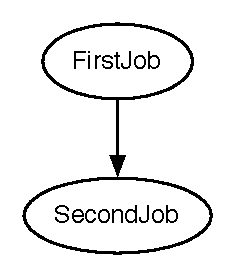
\includegraphics[width=0.25\textwidth]{img/simplest-pipeline}
  \caption{Simplest Job Pipeline, with SecondJob depending on the output of FirstJob (each circle being one Map Reduce Job).}
  \label{fig:simplest-pipeline}
\end{figure}

Such pipeline can be visualised as seen on Figure \ref{fig:simplest-pipeline}, which is an output generated by using the graphviz tool, applied to a file describing the graph as described in the DOT format. The DOT file corresponding to the graph depicted on Figure \ref{fig:simplest-pipeline} is shown in Listing \ref{lst:simplest-pipeline-dot}. DOT descriptions of pipelines are in common use among professionals designing such systems, and can also be generated automatically by Scalding -- which is tremendously useful when working with very long pipelines.

\begin{lstlisting}[caption={Textual description of graph on Figure \ref{fig:simplest-pipeline}, using the DOT graph description language.}, label={lst:simplest-pipeline-dot}]
digraph G {
  1 [label = "FirstJob"];
  2 [label = "SecondJob"];
  
  1->2
}
\end{lstlisting}

The second way of building up pipelines is inside one Scalding Job file. Because of Scalding's rich set of operations, what may look as simple on the surface (for example, the pipeline definition) may have to boil down to multiple Map Reduce Job executions. One obvious case that will cause one Scalding Job to produce multiple Map Reduce Jobs is using data from two separate sources and joining them together. It should be noticed that the notion of ``join'' (as known from relational databases) is something both very powerful and very foreign to Hadoop -- as it is only designed to deal with data in a batch-processing fashion. Scalding allows to express join operations trivially in the the definition file, but it's execution actually is quite complicated and forces all the data from one side of the join to be loaded into Mappers participating in the Job's execution.

\newpage
\begin{lstlisting}[caption={Scalding job, reading data from 2 sources and joining them on dominantColor, producing 3 Map Reduce Jobs}, label={lst:read-and-join-scalding}]
class CompareByDominantColor(args: Args) extends Job(args) {
  // newly analysed video
  val analysedMovieFrames = 
    WritableSequenceFile(input, ("key", "value"))
    .read
    .rename("key", "frame")
    .map(("frame", "value") -> ("dominating", "red", "green", "blue")) { 
        p: (Int, BytesWritable) => calculateHistograms(p._2)
    }
  
  // reference database
  val referenceFrames = 
    HistogramsTable.read
    .rename("dominating", "refDominating")

  // join
  referenceFrames.joinWithSmaller(analysedMovieFrames, 
                                            "dominating" -> "refDominating")
    // operations on joined dataset
}
\end{lstlisting}

Listing \ref{lst:read-and-join-scalding} showcases a simple join operation, which is the core of the algorithms implemented in this thesis. This pipeline definition compiles down into 3 Map Reduce Jobs. It reads from 2 separate data sources, one for the reference data, and one for the currently analysed video. The data for the analysed movie is taken directly from the analysed SequenceFile, containing the frame data. The data of the reference database is read from the \verb|HistogramsTable| which is stored in HBase. The \verb|HistogramsTable| refers to an \textit{HBase Table}, and during the Job's execution will trigger (in this case) a full-scan over the entire ``histograms'' table stored in HBase - in practice it was feasible to sample down the sample count obtained from HBase, by applying the \verb|.sample(75.0)| operation to the larger data set. Figure \ref{fig:3-pipeline} shows the dependencies as modelled by this definition.

\begin{figure}[ch!]
  \centering
  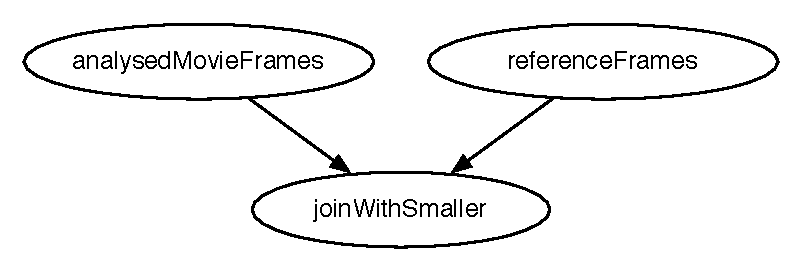
\includegraphics[width=0.75\textwidth]{img/second-simplest-pipeline}
  \caption{Join operation, forcing the Pipeline to consist of 3 Map Reduce Jobs (depicted as circles)}
  \label{fig:3-pipeline}
\end{figure}


The dependencies, as seen on Figure \ref{fig:3-pipeline} between the first two Jobs to the 3rd ``Join Job'' were not explicitly modelled as previously seen using the \verb|next| method, and instead were inferred from the use of the \verb|job1.joinWithSmaller(job2, "key1" -> "key2"| operation. This is very important and useful since:

\begin{itemize}
  \item Cascading is able to determine dependencies between Map Reduce jobs, and execute them on the Hadoop cluster as dictated by their dependency graph.
  \item Jobs that do not depend on each other's outputs can be run in parallel.
\end{itemize}

Thanks to the second property of these Job Pipelines (parallel execution of independent sub-graphs) total execution time of such Map Reduce Pipelines may be further optimised when running on large clusters.

\section{Analyser design summary}
Summing up the Loader's design, it should be clear that most of the architecture required for it's operation is in fact a classical Hadoop cluster. The application itself does not need any additional operational servers, as the only thing the Analyser does is to issue compile Scalding Job descriptions and then send these to the cluster's JobTracker, which takes care of their scheduling and execution. 

The Analyser should be seen as an end-user application. It is run locally on a developers work-station in order to prepare and issue various jobs. This has obvious gains in terms of not requiring the developer's machine to store these humongous amounts of data, and only issue precise queries and jobs.







